\documentclass[12pt]{article}   
\usepackage[utf8]{inputenc}  
\usepackage[russian]{babel}
\usepackage{graphicx}
\usepackage{float}
\usepackage{wrapfig}
\usepackage[letterpaper,top=2cm,bottom=2cm,left=2cm,right=1cm,marginparwidth=1.5cm]{geometry}
\title{Алгоритм ANUBIS}  
\date{Ноябрь 2022}  
\author{Пузевич Роман, Б01-906}

\begin{document}

\maketitle

\section{Введение}
ANUBIS - симметричный блочный криптоалгоритм, разработанный Винсентом Риджменом и Пауло Баррето. ANUBIS является вариантом алгоритма Rijndael. Их объединяет структура типа "квадрат" и набор выполняемых преорбазований. Алгоритм шифрует данные блоками по 16 байтов с ключом размером от 128 до 320 бит с шагом в 32 бита. Анубис был египетским богом бальзамирования и погребения, следовательно, богом "шифрования". Поэтому, по мнению авторов алгоритма, это имя кажется подходящим для шифра.

\subsection{Симметричные криптосистемы}
Прежде чем перейти к алгоритму, рассмотрим симметричные криптосистемы. Симметричная криптосистема - это способ шифрования, в котором, в отличие от асимметричных алгоритмов, для шифрования и расшифрования используется один и тот же ключ. Благодаря этому факту, в сравнении с асимметричными системами, достигается большая простота, большая скорость, меньшая требуемая длина ключа, более простая реализация. Но так же у подобных алгоритмов есть существенный недостаток: необходим защищенный канал для передачи ключа.

\begin{figure}[h]
    \centering
    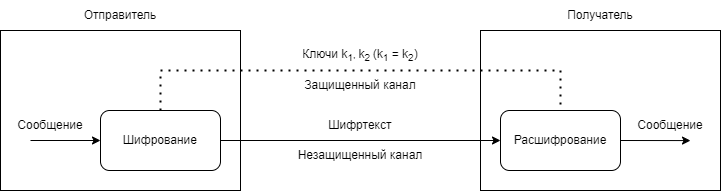
\includegraphics[width=0.8\linewidth]{scheme.png}
    \caption{Симметричная криптосистема}
    \label{fig:scheme}
\end{figure}

\section{Алгоритм}
Теперь рассмотрим сам алгоритм. Алгоритм представляет блок данных в виде 16-байтового массива $M_{4x4}[GF(2^{8})]$ (все вычисления производятся в конечном поле Галуа):

\begin{figure}[h]
    \centering
    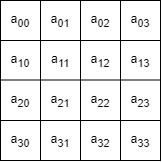
\includegraphics[width=0.18\linewidth]{matrix.png}
    \caption{Представление данных в алгоритме}
    \label{fig:scheme}
\end{figure}
\newline
В каждой итерации алгоритма выполняются действия:

\subsection{Первая операция}
Табличная замена $\gamma$ -- отображение $M_{4x4}[GF(2^{8})] \to M_{4x4}[GF(2^{8})]$ (или $M_{Nx4}[GF(2^{8})] \to M_{Nx4}[GF(2^{8})]$ в общем случае): \newline
$b_{ij} = S(a_{ij})$

\begin{figure}[h]
    \centering
    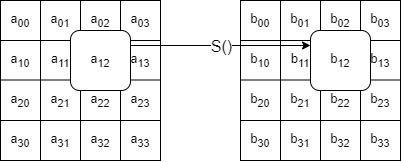
\includegraphics[width=0.4\linewidth]{first_function.png}
    \caption{Первое преобразование}
    \label{fig:scheme}
\end{figure}
\newline
Псевдослучайные значения таблицы выбраны так, чтобы они удовлетворяли следующему свойству:
$S(S(x)) = x, \forall x \in GF(2^{8})$


\subsection{Вторая операция}
Байтовая перестановка $\tau$ -- отображение $M_{4x4}[GF(2^{8})] \to M_{4x4}[GF(2^{8})]$: \newline
$c_{ij} = b_{ji}$, где $b_{ij}$ результат выполнения предыдущей операции.

\begin{figure}[h]
    \centering
    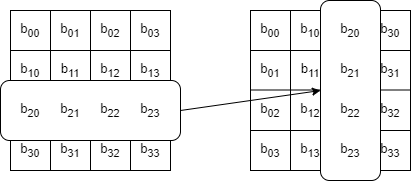
\includegraphics[width=0.4\linewidth]{second_func.png}
    \caption{Второе преобразование}
    \label{fig:scheme}
\end{figure}

\newline
Данную операцию можно воспринимать как транспонирование исходного блока данных.

\subsection{Третья операция}
Матричное умножение $\theta$ -- отображение $M_{4x4}[GF(2^{8})] \to M_{4x4}[GF(2^{8})]$ (или $M_{Nx4}[GF(2^{8})] \to M_{Nx4}[GF(2^{8})]$ в общем случае): \newline
$D = CH$
\newline
В этой операции мы умножаем результат предыдущих операций на постоянную матрицу H (умножение производится в конечном поле $GF(2^{8})$):

\[H = \left(
    \begin{array}{cccc}
    1 & 2 & 4 & 6\\
    2 & 1 & 6 & 4\\
    4 & 6 & 1 & 2\\
    6 & 4 & 2 & 1
    \end{array}
\right)\]


\subsection{Последняя операция}
Нахожение ключа $\sigma$ - отображение $M_{4x4}[GF(2^{8})] \to M_{4x4}[GF(2^{8})]$ (или $M_{Nx4}[GF(2^{8})] \to M_{Nx4}[GF(2^{8})]$ в общем случае): \newline
$e_{ij} = d_{ij} \oplus K^{r}_{ij}$

\begin{figure}[h]
    \centering
    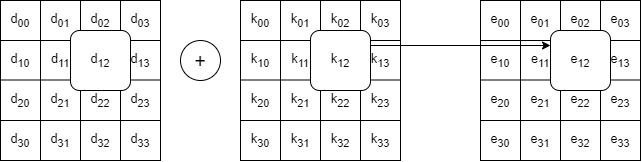
\includegraphics[width=0.7\linewidth]{last_func.png}
    \caption{Последнее преобразование}
    \label{fig:scheme}
\end{figure}

\newline
В данной операции мы побитово накладываем ключ r-го раунда $K^{r}$ на каждый из байтов матрицы, получившейся после предыдущих операций. 
\newline
\newline
Перечисленные операции выполняются в заданной последовательности ($\gamma, \tau, \theta, \sigma$) во всех раундах, кроме последнего. В последнем раунде не выполняется операция $\theta$. Более того, перед первым раундом выполняется "входное отбеливание" данных путем наложения нулевого ключа с помощью операции XOR. Перечисленные операции обратимы, то есть расшифрование происходит в обратном порядке шифрования.
Количество раундов шифрования R определяется размером ключа и вычисляется следующим образом: $R = 8 + N$, где N размер ключа в 4-байтовых фрагментах.


\section{Генерация ключа}
В данном разделе мы затронем то, как мы получим ключ, с помощью которого будем шифровать данные, из исходного ключа. Ключ у нас может быть больше массива данных, поэтому необходимо привести его к такому же виду, как и шифруемый блок данных. Стоит упомянуть то, как мы будем представлять наш ключ в процессе шифрования. Ключ представляется в виде $4N$-байтовго массива $M_{Nx4}[GF(2^{8})]$

\begin{figure}[h]
    \centering
    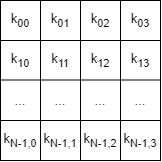
\includegraphics[width=0.18\linewidth]{key.png}
    \caption{Представление ключа в алгоритме}
    \label{fig:scheme}
\end{figure}
% мб добавить картинку, или убрать в самом начале

\subsection{Вычисление вспомогательных ключей}
В самом начале вычислим вспомогательные ключи, которые понадобятся для нахождения основных ключей шифрования. Количество вспомогательных ключей зависит от того, сколько раундов шифрования у нас будет. Процедура их нахождения рекурсивная, поэтому определим нулевой член рекурсии:

\begin{enumerate}
    \item Нулевым вспомогательным ключом будет являться исходный ключ шифрования $K \in GF(2^{8})^{4N}, 
    
    3 < N < 11$:

  
    \[k^{0} = K \]
    \item Рекуррентная формула для нахождения вспомогательных ключей: 
    \[k^{r} = (\sigma(c^{r}) \cdot \theta \cdot \pi \cdot \gamma)(k^{r-1}), r > 0 \]
\end{enumerate}
\newline
Рассмотрим операции, которые выполняются для генерации вспомогательных ключей.
\begin{enumerate}
    \item Операция $\gamma$ аналогична той, которую мы рассматривали в пункте 2.1: $B = \gamma(A)$
    \item Операция $\pi$ является циклическим сдвигом. В данной операции столбец матрицы циклически сдвигается вниз в зависимости от номера столбца, j-ый столбец циклически сдвигается вниз на j позиций: $\pi(B) = C \leftrightarrow c_{ij} = b_{(i-j)modN, j}, 0 \leq i \leq N - 1, 0 \leq j \leq 3$
    
    \begin{figure}[h]
        \centering
        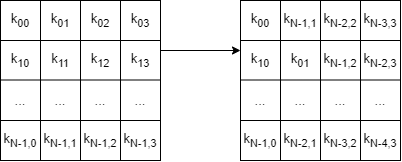
\includegraphics[width=0.4\linewidth]{operation_pi.png}
        \caption{Операция $\pi$}
        \label{fig:scheme}
    \end{figure}
    
    \item Операция $\theta$ аналогична той, которую мы рассматривали в пункте 2.3: $D = \theta(C)$
    \item Операция $\gamma$ аналогична той, которую мы рассматривали в пункте 2.4, но вместо ключа используется матрица $c^{r}$. Матрица $c^{r} \in M_{Nx4}[GF(2^{8})], 4 \leq N \leq 10$ определяется следующим образом:
\[c^{r}_{0,j} = S[4(r-1) + j], 0 \leq j \leq 3\]
\[c^{r}_{i,j} = 0, 1 \leq i < N, 0 \leq j \leq 3\]
, где S - табличная замена из пункта 2.1, а r - раунд шифрования

% табличка 
\end{enumerate}


\subsection{Основной ключ}
Теперь рассмотрим, как генерируется основной ключ из вспомогательного. Алгоритм выглядит следующим образом:
\[K^{r} = (\tau \cdot \omega \cdot \gamma)(k^{r}), 0 \leq r \leq R;\]
\newline
Рассмотрим операции, которые выполняются для генерации основного ключа:
\begin{enumerate}
    \item Операция $\gamma$ аналогична той, которую мы рассматривали в пункте 2.1: $B = \gamma(A)$
    \item Операция $\omega$ - операция извлечения ключа. Она представляет собой линейное отображение основанное на матрице $V \in M_{4xN}[GF(2^{8})]$:
    \[V = \left(
        \begin{array}{ccccc}
        1 & 1 & 1 & \ldots & 1\\
        1 & 2 & 2^{2} & \ldots & 2^{N-1}\\
        1 & 6 & 6^{2} & \ldots & 6^{N-1}\\
        1 & 8 & 8^{2} & \ldots & 8^{N-1}
        \end{array}
    \right))\]
    \item Операция $\tau$ аналогична той, которую мы рассматривали в пункте 2.2: $D = \tau(C)$
\end{enumerate}
\newline
На выходе мы получаем ключ размером 4x4 байта.


\section{Криптостойкость}
Перед тем, как говорить о безопасности алгоритма, введем понятия, связанные с безопасностью.

\subsection{K-безопасность}
Блочный шифр является K-безопасным, если все возможные типы атак на него имеют то же ожидаемое время и требования к хранению, что и для большинства возможных блочных шифров с одинаковыми размерами. Это должно иметь место для всех возможных режимов доступа для криптоаналитика и для любого априорного распределения ключей.
K-безопасность -- это, по сути, относительная мера. Вполне возможно построить K-безопасный блочный шифр с 5-битными блоком данных и длиной ключа. Недостаток безопасности, обеспечиваемый такой схемой, обусловлен ее небольшими размерами, а не тем фактом, что схема не соответствует требованиям, предъявляемым этими размерами. Очевидно, что чем длиннее ключ, тем выше требования к безопасности.

\subsection{Герметичный блочный шифр}
Можно представить себе шифры, которые имеют определенные слабые места и все еще являются K-безопасными. По этим причинам введем еще одно понятие безопасности.
Блочный шифр является герметичным, если у него нет слабых мест, которых нет у большинства блочных шифров с одинаковой длиной блока и ключа. Другими словами, блочный шифр является герметичным, если его внутренняя структура не может быть использована при какой-либо атаке.

Для всех разрешенных длин ключей ANUBIS является:
\newline
- К-безопасным;
\newline
- Герметичным.
\newline
Ожидается, что для всех определенных длин ключей Anubis будет вести себя так же, как и другой блочный шифр с заданными длинами блока данных и ключа (в смысле K-безопасности и Герметичности). Это подразумевает, среди прочего, следующее: наиболее эффективной атакой по восстановлению ключей для ANUBIS является атака полным перебором. Получение информации из заданных пар открытый текст/зашифрованный текст о других парах открытый текст/зашифрованный текст не может быть выполнено более эффективно, чем путем определения ключа путем полного перебора. Ожидаемая сложность полного перебора ключа зависит от длины ключа шифрования и равна $2^{m-1}$ для $m$-битного ключа. 

\section{Эффективность алгоритма}

\subsection{Генерация ключа}
В таблице приведена скорость генерации ключа. Генерация ключа реализована с помощью "модифицированной" таблицы S (данная таблица используется в операции $\gamma$). Модификация заключается в том, что после операции $\gamma$ идет операция $\omega$, поэтому таблицу S можно немного модифицировать с учетом умножения на матрицу V. Объем памяти, необходимый для хранения "модифицированной" таблицы S: 2 Мбайта.

\begin{center}
\begin{tabular}{|c|c|c|}
    \hline
    Размер ключа, бит & Циклы (шифрование) & Циклы (расшифрование) \\
    \hline
    $128$ & $3352$ & $4527$ \\
    \hline
    $160$ & $4445$ & $5709$ \\
    \hline
    $192$ & $6644$ & $8008$ \\
    \hline
    $224$ & $8129$ & $9576$ \\
    \hline
    $256$ & $9697$ & $11264$ \\
    \hline
    $288$ & $11385$ & $12931$ \\
    \hline
    $320$ & $13475$ & $15169$ \\
    \hline
\end{tabular}
\end{center}

Более дорогая стоимость генерация ключей для расшифрования обусловлена операцией $\theta$ для ключей $R-1$ раунда

\subsection{Шифрование и расшифрование}
Поскольку ANUBIS имеет инволюционную структуру, то шифрование и расшифрование одинаково эффективны для любого количества раундов. Кроме этого для процедур шифрования и расшифрования также используется "модифицированная" таблица S, только уже с учетом матрицы H. В таблице приведена скорость на процессоре Intel Core i7-12700K:

\begin{center}
\begin{tabular}{|c|c|c|c|}
    \hline
    Размер ключа, бит & Циклы/байт & Циклы/блок & Мбит/с \\
    \hline
    $128$ & $36.8$ & $589$ & $793$ \\
    \hline
    $160$ & $39.3$ & $628$ & $744$ \\
    \hline
    $192$ & $41.6$ & $665$ & $703$ \\
    \hline
    $224$ & $43.8$ & $701$ & $667$ \\
    \hline
    $256$ & $46.3$ & $740$ & $631$ \\
    \hline
    $288$ & $48.5$ & $776$ & $602$ \\
    \hline
    $320$ & $50.8$ & $813$ & $575$ \\
    \hline
\end{tabular}
\end{center}

\section{Достоинства и недостатки}
Рассмотрим достоинства алгоритма:
\begin{enumerate}
    \item Аппаратное. ANUBIS довольно быстрый алгоритм. При этом он не требует большого объема памяти (как для кода, так и для вспомогательных таблиц). Кроме того, есть возможность параллельного исполнения (можно вычислять ключи параллельно с шифротекстом/открытым текстом).
    \item Инволюционная структура. Тот факт, что все компоненты алгоритма ANUBIS являются инволюциями, уменьшает размер кода, который осуществляет шифрование/расшифрование.
    \item Сложная генерация ключей. Преимуществом является повышенная устойчивость к атакам на ключи.
\end{enumerate}
\newline
Рассмотрим недостатки алгоритма:
\begin{enumerate}
    \item Медленная генерация ключей. За устойчивость к атакам приходится платить скоростью. Но несмотря на это алгоритм все еще остается довольно быстрым.
    \item ANUBIS схож с другим блочным криптоалгоритмом Rijndael (он является стандартом шифрования в США). Но несмотря на его схожесть, он не имеет серьезных преимуществ перед Rijndael. Поэтому он не используется как стандарт.
\end{enumerate}

\section{Заключение}
В работе рассмотрен алгоритм ANUBIS. Данный алгоритм обеспечивает быстрое и надежное шифрование. На конкурсе NESSIE он был признан одним из самых быстрых и криптостойких алгоритмов. Если бы не большое сходство с Rinjdael, он мог бы быть стандартом шифрования в США.

\section{Ссылки}
\begin{enumerate}
    \item https://web.archive.org/web/20160606112246/http://www.larc.usp.br/~pbarreto/AnubisPage.html
    \item 
    https://www.phantastike.com/encryption/algoritmy$\verb|_|$shifrovaniya/djvu/view/
    \item https://ru.wikipedia.org/wiki/%D0%A1%D0%B8%D0%BC%D0%BC%D0%B5%D1%82%D1%80%D0%B8%D1%87%D0%BD%D1%8B%D0%B5_%D0%BA%D1%80%D0%B8%D0%BF%D1%82%D0%BE%D1%81%D0%B8%D1%81%D1%82%D0%B5%D0%BC%D1%8B
    \item https://ru.wikipedia.org/wiki/%D0%91%D0%BB%D0%BE%D1%87%D0%BD%D1%8B%D0%B9_%D1%88%D0%B8%D1%84%D1%80#%D0%90%D1%82%D0%B0%D0%BA%D0%B0_%D0%BF%D0%BE%D0%BB%D0%BD%D1%8B%D0%BC_%D0%BF%D0%B5%D1%80%D0%B5%D0%B1%D0%BE%D1%80%D0%BE%D0%BC
\end{enumerate}
\end{document}
